\section{处理辐射积分}\label{sec:处理辐射积分}

渲染中最频繁的任务之一就是求辐射度量数量的积分。
本节中,我们将介绍可以使该任务更简单的一些技巧。
为了说明这些技术的运用,我们将以计算在一点处的辐射照度为例。
在曲面法线为$\bm n$的点$\bm p$处的辐射照度取决于
方向集$\Omega$上的辐射亮度即
\begin{align}\label{eq:5.4}
    E({\bm p},{\bm n})=\int\limits_{\Omega}{L_{\mathrm{i}}({\bm p},{\bm\omega})|\cos\theta|\mathrm{d}\bm\omega}\, ,
\end{align}
其中$L_{\mathrm{i}}({\bm p},{\bm\omega})$是入射辐亮度函数(\reffig{5.12})
而该积分中项$\cos\theta$取决于辐射亮度定义中的项$\mathrm{d}A^{\perp}$。
$\theta$度量$\bm\omega$和曲面法线$\bm n$之间的夹角。
辐射照度通常在关于给定曲面法线$\bm n$的半球方向$H^2(\bm n)$上算出。
\begin{figure}[htbp]
    \centering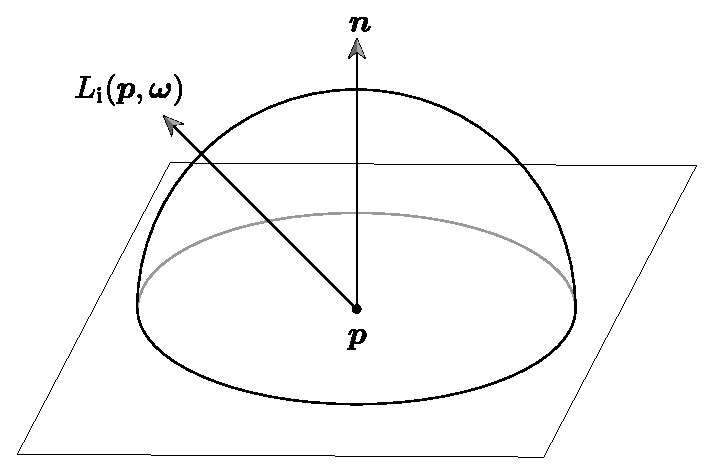
\includegraphics[width=0.5\linewidth]{chap05/Irradiancefromradiance.eps}
    \caption{点$\bm p$处的辐射照度由辐射亮度乘以在该点上整个上半球入射方向余弦的积分得到。}
    \label{fig:5.12}
\end{figure}

\subsection{投影立体角上的积分}\label{sub:投影立体角上的积分}
辐射度量数量积分中的各种余弦常常和积分学中的解释搞混。
这个问题可通过用\keyindex{投影立体角}{projected solid angle}{solid angle立体角}而不是
立体角度量积分所需的物体所对面积来避免。
物体所对的投影立体角通过将该物体投影到单位球上决定,
这和立体角的做法一样,但接着要将所得形状再向下投影到
垂直于曲面法线的单位圆盘上(\reffig{5.13})。
半球方向上关于余弦加权的立体角积分可重写为在投影立体角上的积分。
\begin{figure}[htbp]
    \centering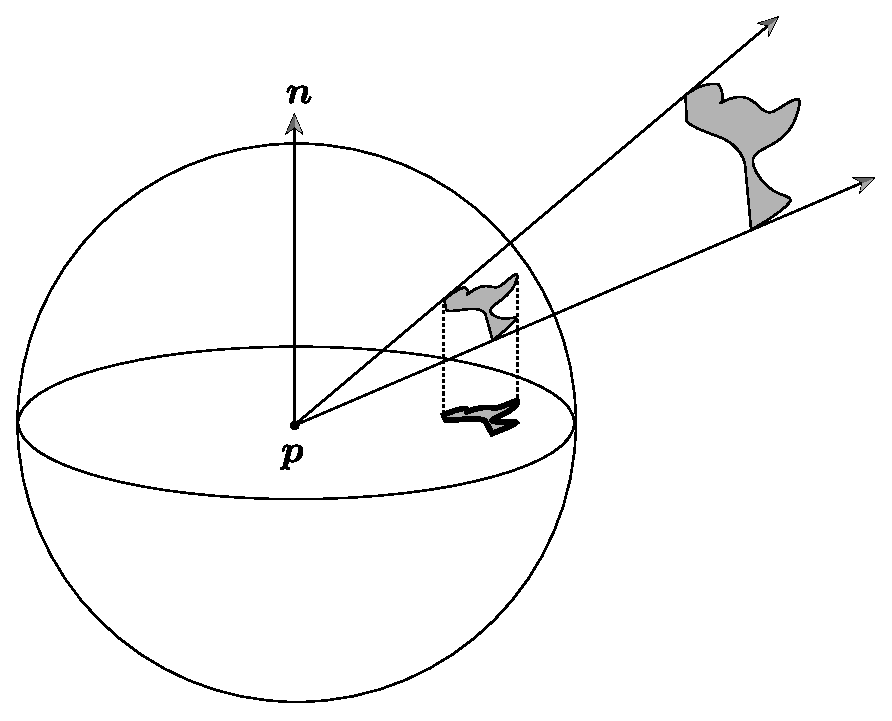
\includegraphics[width=0.6\linewidth]{chap05/Projectedsolidangle.eps}
    \caption{物体所对的投影立体角是其所对的余弦加权立体角。
        通过求物体的立体角、将其向下投影到垂直于曲面法线的平面上并
        度量该区域的面积可以将其算出。因此投影立体角取决于
        计算处的曲面法线,因为法线朝着平面投影方向。}
    \label{fig:5.13}
\end{figure}

投影立体角度量与立体角度量的关系为
\begin{align*}
    \mathrm{d}{\bm\omega}^{\perp}=|\cos\theta|\mathrm{d}{\bm\omega}\, ,
\end{align*}
所以在半球上由辐射亮度计算辐射照度的积分可更简单地重写为
\begin{align*}
    E({\bm p},{\bm\omega})=\int\limits_{H^2({\bm n})}{L_{\mathrm{i}}({\bm p},{\bm\omega})\mathrm{d}{\bm\omega}^{\perp}}\, .
\end{align*}

对于本书剩余部分,我们会以立体角而不是投影立体角的形式书写方向上的积分。
然而在其他资源中,可能会用投影立体角,所以弄清被积分式实际的度量总是很重要的。

正如我们用入射辐亮度求辐射照度那样,我们也可以通过在物体表面积$A$上积分
来计算从某物体向法线周围半球发出的总通量:
\begin{align*}
    \varPhi & =\int\limits_A{\int\limits_{H^2({\bm n})}L_{\mathrm{o}}({\bm p},{\bm\omega})\cos\theta\mathrm{d}{\bm\omega}\mathrm{d}A}   \\
            & =\int\limits_A{\int\limits_{H^2({\bm n})}L_{\mathrm{o}}({\bm p},{\bm\omega})\mathrm{d}{\bm\omega}^{\perp}\mathrm{d}A}\, .
\end{align*}

\subsection{球坐标上的积分}
将立体角上的积分转化到球面坐标$(\theta,\varphi)$上常常很方便。
回想一个$(x,y,z)$方向坐标也可写成球面角形式(\reffig{5.14})
\sidenote{译者注:原书此图和后续图中标注为$\varphi$,该公式和后续公式则使用$\phi$。
    笔者修改为统一使用$\varphi$,与前面的章节照应。}:
\begin{align*}
    x & =\sin\theta\cos\varphi\, , \\
    y & =\sin\theta\sin\varphi\, , \\
    z & =\cos\theta\, .
\end{align*}
\begin{figure}[htbp]
    \centering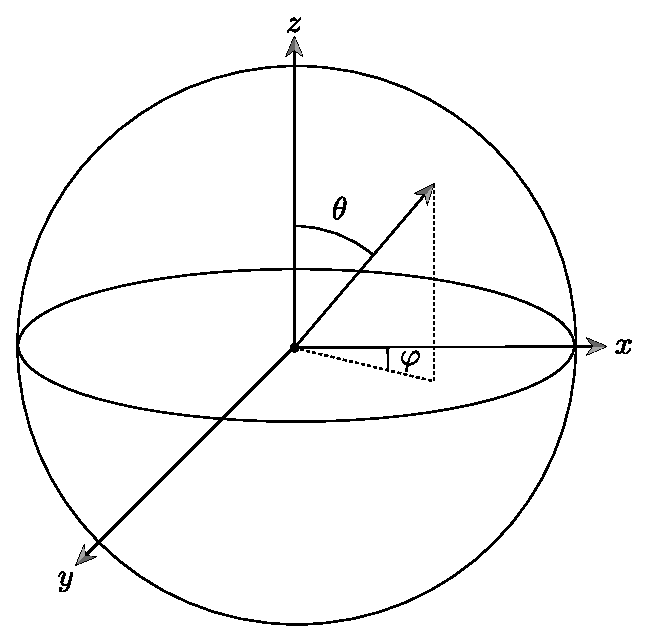
\includegraphics[width=0.5\linewidth]{chap05/Sphericalcoordinates.eps}
    \caption{如果也给出了基向量$x,y$和$z$,则方向向量也可写作球面坐标$(\theta,\varphi)$的形式。
        球面角公式让两者之间的转化很容易。}
    \label{fig:5.14}
\end{figure}

为了将立体角上的积分转化为$(\theta,\varphi)$上的积分,
我们需要能表达方向集的微分面积$\mathrm{d}\bm\omega$
与$(\theta,\varphi)$的微分面积之间的关系(\reffig{5.15})。
微分面积$\mathrm{d}\bm\omega$是其边的
微分长度$\sin\theta\mathrm{d}\varphi$和$\mathrm{d}\theta$之积。因此,
\begin{align}\label{eq:5.5}
    \mathrm{d}{\bm\omega}=\sin\theta\mathrm{d}\theta\mathrm{d}\varphi\, .
\end{align}
\begin{figure}[htbp]
    \centering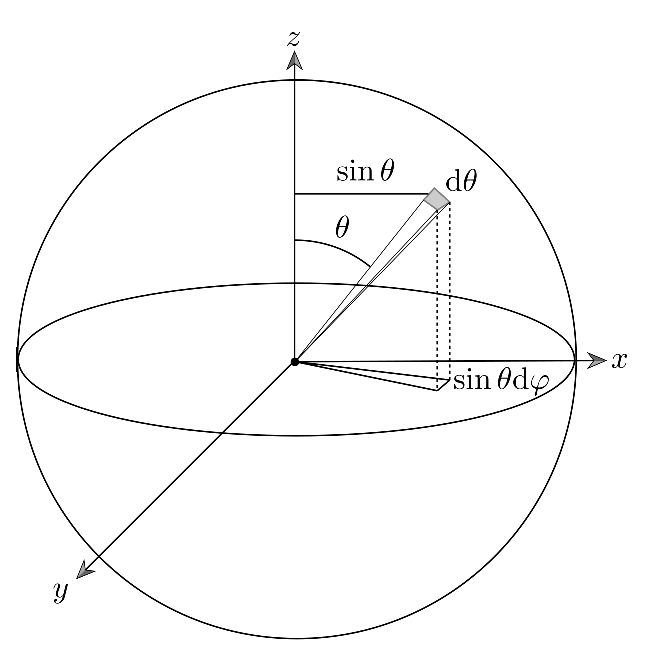
\includegraphics[width=0.5\linewidth]{chap05/Sindthetadphi.eps}
    \caption{一个微分立体角所对的微分面积$\mathrm{d}\bm\omega$是
        两边微分长度$\sin\theta\mathrm{d}\varphi$和$\mathrm{d}\theta$的积。
        得到的关系$\mathrm{d}{\bm\omega}=\sin\theta\mathrm{d}\theta\mathrm{d}\varphi$是
        在立体角上的积分和球面角上的积分之间转化的关键。}
    \label{fig:5.15}
\end{figure}

因此我们可以看到在半球上的辐射照度积分,即$\Omega=H^2({\bm n})$的\refeq{5.4},
可以等价地写为
\begin{align*}
    E({\bm p},{\bm\omega})=\int_0^{2\pi}\int_0^{\frac{\pi}{2}}L_{\mathrm{i}}({\bm p},\theta,\varphi)\cos\theta\sin\theta\mathrm{d}\theta\mathrm{d}\varphi\, .
\end{align*}
如果来自所有方向的辐射亮度都相同,则等式简化为$E=\pi L_{\mathrm{i}}$。

为了方便,我们将定义两个把$\theta$和$\varphi$转化为$(x,y,z)$方向向量的函数。

